\documentclass[journal]{IEEEtran}
\usepackage{amsthm}
\usepackage{url}
\usepackage{graphicx}
\usepackage{hyperref}

\begin{document}
\onecolumn
\title{Clubs Web Portal}

\author{

Chirag Khurana\\
\href{mailto:2016csb1037@iitrpr.ac.in}{2016csb1037@iitrpr.ac.in}

}
\maketitle
\section{Objective}
To make a web portal for various clubs of our institute. Through which each member will be officially registered and we will have records of whats going on, who did what, what is pending, etc.

\section{Design}
It will be like Facebook except chatting. It will have-
\begin{itemize}
\item News Feed
\item Users (can log-in with Google)
\item Club Representatives
\item Membership Request (will be accepted by Representatives)
\item Subscription to the channels of the club for public
\item Projects under the club
\item Notifications
\item Feedback
\end{itemize}
It can be further extended for Android app with same features.

\section{Schema}
\centering
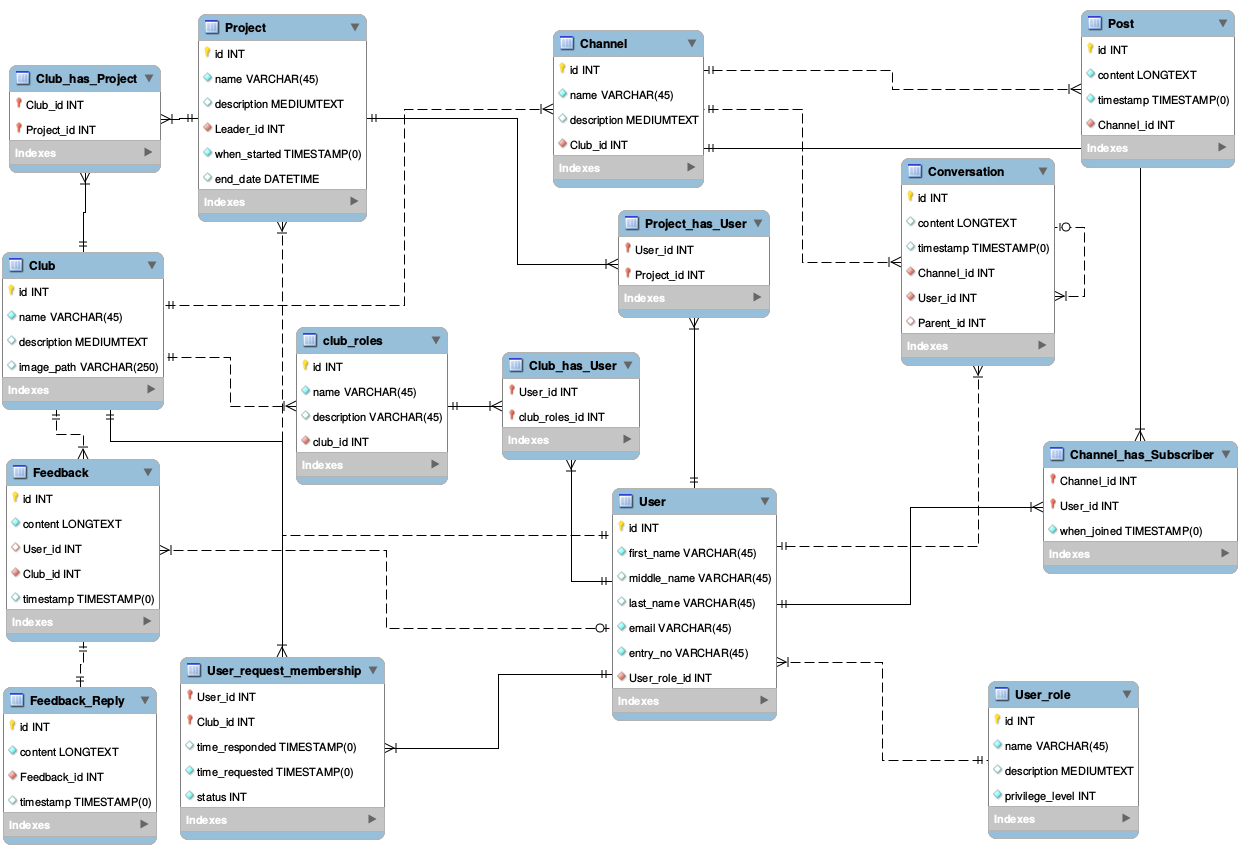
\includegraphics[width=1\linewidth]{schema.png}

\end{document}

